Using logic grid puzzles as a use-case, we validate the feasibility of finding non-redundant explanation sequences and generating nested explanation sequences.
As data, we use puzzles from Puzzle Baron’s Logic Puzzles Volume 3~\cite{logigrammen}.
The first 10 puzzles were used to construct the grammar; the next 10 to test the genericity of the grammar.
%\bart{In onze experiementen hebben we acht (+1) puzzels. Is daar een reden voor??? Ik zou tien verwachten (ofwel de eerste ofwel de laatste tien...}
Our experiments below are on test puzzles only; we also report results on the \textit{pasta} puzzle, which was sent to us by someone who did not manage to solve it himself.

As constraint solving engine, we use \idp~\cite{IDP} due to the variety of inference methods it supports natively.
The algorithms themselves are written in embedded LUA, which provides an imperative environment inside the otherwise declarative \idp system.
The code was not optimized for efficiency and can at this point not be used in an interactive setting, as it takes between 15 minutes to a few hours to fully explain a logic grid puzzle.
Experiments were run on an Intel(R) Xeon(R) CPU E3-1225 with 4 cores and 32 Gb memory, running linux 4.15.0 and \idp 3.7.1.



%\bart{
	%Volgens mij kloppen de kolommen \textbf{\% clue} \& \textbf{\% clue+i.} niet. 
	%Experimenten opnieuw gerund met juiste size functie??? 
%Ik heb in de size het ``foute'' stuk in commentaar (``Special case'') gezet: 
%} 
%\tias{ook, avg cost is niet >100} 
%\bart{Good catch: alle costs nakijken dat ze correct zijn. Maar die average, klopt ide niet? 80 procent van de stappen zijn wel bijectivity of trans met kost van plusminus 5-10}


\begin{table}[t]
	\centering
	\resizebox{\textwidth}{!}{%
	\begin{tabular}{c|ccc|cc|cccccc}
		\textbf{p} & \textbf{$|$types$|$} & \textbf{$|$dom$|$} & \textbf{$|$grid$|$} & \textbf{\# steps} & $\overline{\text{\textbf{cost}}}$ & \textbf{1 bij.} & \textbf{1 trans.} & \textbf{1 clue} & \textbf{1 clue+1i.} & \textbf{1 clue+ $>$1i.} & \textbf{mult i.} \\\hline %& \textbf{mult c.} \\\hline
		1 &       4 &            5 &         150 &    112 &      27.06 &  31.25\% &  50.00\% &    0.89\% &      7.14\% &  10.71\%  &  0.00\% \\ %  &  0.00\%  \\
		2 &       4 &            5 &         150 &    119 &      27.77 &  23.53\% &  57.14\% &    1.68\% &      7.56\% &  10.08\%  &  0.00\% \\ %  &  0.00\%  \\
		3 &       4 &            5 &         150 &    110 &      23.93 &  32.73\% &  51.82\% &    0.00\% &      2.73\% &  12.73\%  &  0.00\% \\ %  &  0.00\%  \\
		4 &       4 &            5 &         150 &    115 &      24.54 &  27.83\% &  55.65\% &    2.61\% &      7.83\% &   6.09\%  &  0.00\% \\ %  &  0.00\%  \\
		5 &       4 &            5 &         150 &    122 &      24.97 &  24.59\% &  59.02\% &    0.82\% &      4.10\% &  11.48\%  &  0.00\% \\ %  &  0.00\%  \\
		6 &       4 &            5 &         150 &    115 &      22.58 &  26.96\% &  58.26\% &    2.61\% &      6.09\% &   6.09\%  &  0.00\% \\ %  &  0.00\%  \\
		7 &       4 &            5 &         150 &    110 &      26.79 &  35.45\% &  46.36\% &    0.91\% &      8.18\% &   9.09\%  &  0.00\% \\ %  &  0.00\%  \\
		8 &       4 &            5 &         150 &    118 &      26.81 &  33.90\% &  47.46\% &    3.39\% &      5.08\% &  10.17\%  &  0.00\% \\ %  &  0.00\%  \\
		9 &       4 &            5 &         150 &    114 &      24.75 &  28.95\% &  54.39\% &    3.51\% &      3.51\% &   9.65\%  &  0.00\% \\ %  &  0.00\%  \\
		p &       4 &            4 &          96 &     83 &      34.45 &  33.73\% &  40.96\% &    1.20\% &      4.82\% &  16.87\%  &  2.41\% %  &  0.00\%
	\end{tabular}
	}
	\caption{Properties of the puzzles, explanation sequences and constraints used in the explanations.}
	\label{table:composition}
\end{table}


\myparagraph{Sequence composition}
We first investigate the properties of the puzzles and the composition of the resulting sequence explanations. The results are shown in Table~\ref{table:composition}. The first column is the puzzle identifier, where the puzzle identified as p is the pasta puzzle, our running example. 
% The next column shows the configuration of the puzzle as a tuple of 3 numbers: the number of types (e.g. person, sauce); the number of entities of each type; and the number of cells in the grid, i.e.\ the number of literals in the maximal consequence interpretation $I_n=max(\emptyset, \allconstraints)$.
\emilio{hard to fit everything inside ...}
The next 3 columns show properties of the puzzle:
$|type|$ is the number of types (e.g. person, sauce) while $|dom|$ is the number of entities of each type and $|grid|$ is the number of cells in the grid, i.e.\ the number of literals in the maximal consequence interpretation $I_n=max(\emptyset, \allconstraints)$.
Coincidentally, almost all the puzzles have 4 types with domain size 5,  hence 150 cells, except for the pasta puzzle which has a domain size of 4, thus 96 cells.

Columns 5 and 6 show the amount of steps ($\# steps$) in the explanation sequences found, and $\overline{cost}$ is the average cost of an explanation step in the puzzle. The number of inference steps is around 110-120 for all but the pasta puzzle, which is related to the grid size.

The rest of the columns investigate the proportion of inference steps in the explanation sequence, e.g. the trivia steps using just one bijection constraint (\textbf{1 bij.}), one transitivity constraint (\textbf{1 trans.}) or one clue (\textbf{1 clue}) and no other constraints; and the more complex inference steps using one clue and some implicit (bijectivity or transitivity) constraint (\textbf{1 clue+i}), multiple implicit constraints (\textbf{mult i.}). 
We see that while our method can combine multiple clues, the explanations generated never require combining multiple clues in one inference step, that is, the method always find simpler steps involving just one clue. 
Therefore, we omit reporting multiple clues with other constraints. 
We can observe that around 25-30\% of steps are simple bijectivity steps (e.g. completing a row or column in one relation), around 50\% are transitivity steps and 10-15\% use just a single clue. 
The remaining 5-10\% use a more complex combination of a clue with other constraints. 
Also notably, the puzzles from the booklet never require combining implicit constraints, while the harder pasta puzzle does. 
In general, less then $1/5$th of the explanations actually need to use a clue or a combination of a clue and implicit constraints.
%\emilio{add resutls here: waiting for the new results}
%\todo{ADD THE DIFFERENT TYPES OF CLUE AND EXPLAIN. Also: should be reran? --> add clue vs clue+1 implicit vs clue +2implicit}

%In the table, \#m-i and \#m-c refer to the use of multiple implicit constraints and multiple clues respectively.
%We can see that it is never necessary to combine multiple clues in one inference step.
%Also, notably, the puzzles from the booklet never require combining implicit constraints, while the anecdotally hard pasta puzzle is the only one that does: it cannot be solved by focussing on the clues but requires combining facts and knowledge in the table alone to crack it.

\myparagraph{Sequence progression}
The left side of Figure \ref{fig:steps} on page~\pageref{fig:steps} shows a visualisation of the type of explanation used in each of the explanation steps for puzzles 1,2,5 and p. 
We can see that typically at the beginning of the sequence, individual clues (3rd line) and some individual bijectivity (1st line) and transitivity (2nd line) constraints are used, i.e., trivial ones.\tias{Ideally, you would reuse the column names I've put in the above table now...; also can the background lines be less prominent? perhaps half-transparent or light gray or so. Also, I would do prefer that m-i is the top line because it is so 'special'...}
This is then followed by a series of clues that also involve bijectivity/transitivity constraints, after which a large fraction of the table can be completed with bijectivity/transitivity, followed by a few last clue/implicit constraint combinations and another round of completion.
The exception to this is the pasta puzzle.
We can see that after around 20 steps where mostly clues have been used, twice\tias{is this twice? not clear in visu, looks like once} a combination of implicit logigram constraints must be used to derive a new fact, after which the table can be easily completed with bijectivity/transitivity and twice the use of a clue.


% \ourfigure % \emilio{wat is ourfigure ? } \tias{a command of figures defined lower, outdated I assume}
\begin{table}[t]
	\centering
	\begin{tabular}{l|c|cccc|ccccc}
		  & \multicolumn{5}{c|}{\bf average nr. of facts used} & \multicolumn{5}{c}{\bf \% of explanations with a clue that use \# facts}                                                                                \\
		p & all &  Bij. & Trans. &  Clue & multi i. & 0 facts & 1 facts & 2 facts & 3 facts & $\>$3 facts \\\hline
		1 &  1.84 &  2.37 &   2.00 &  0.52 &        - &  66.67\% &  28.57\% &   0.00\% &   0.00\% &    4.76\% \\
		2 &  1.85 &  2.50 &   2.00 &  0.61 &        - &  47.83\% &  47.83\% &   0.00\% &   4.35\% &    0.00\% \\
		3 &  1.84 &  2.33 &   2.00 &  0.24 &        - &  82.35\% &  11.76\% &   5.88\% &   0.00\% &    0.00\% \\
		4 &  1.89 &  2.50 &   2.00 &  0.47 &        - &  68.42\% &  15.79\% &  15.79\% &   0.00\% &    0.00\% \\
		5 &  1.85 &  2.50 &   2.00 &  0.35 &        - &  65.00\% &  35.00\% &   0.00\% &   0.00\% &    0.00\% \\
		6 &  1.84 &  2.35 &   2.00 &  0.29 &        - &  76.47\% &  17.65\% &   5.88\% &   0.00\% &    0.00\% \\
		7 &  1.88 &  2.31 &   2.00 &  0.75 &        - &  55.00\% &  25.00\% &  10.00\% &  10.00\% &    0.00\% \\
		8 &  1.86 &  2.58 &   2.00 &  0.18 &        - &  81.82\% &  18.18\% &   0.00\% &   0.00\% &    0.00\% \\
		9 &  1.85 &  2.45 &   2.00 &  0.32 &        - &  78.95\% &  15.79\% &   0.00\% &   5.26\% &    0.00\% \\
		p &  1.73 &  2.07 &   2.00 &  0.53 &     4.00 &  68.42\% &  21.05\% &   0.00\% &  10.53\% &    0.00\% \\
	\end{tabular}
	\caption{Statistics on number of previously derived facts $|E|$ used in the explanation steps.\tias{pls change order to: all, bij. trans. clue, m-i}}
 	\label{table:sequence_leve}
\end{table}
\myparagraph{Explanation size}
Our cost-function is constructed to favour few (if any) clues and constraints in the explanations, and a small number of previously derived facts $|E|$.
Table~\ref{table:sequence_leve}, first 6 columns, shows the average number of facts used per type of constraints used in the explanation.
We can observe that the average number of facts used is indeed low, less than two (column 'all').
The breakdown per type of constraint shows that bijectivity typically uses more facts: it either uses three `negative' facts in one row to infer a `positive' fact, as in Figure~\ref{fig:zebrascreen} or it uses one `positive' fact to infer three negative facts.
Note that for such an intuitive constraint, the number of facts used does not matter much. Transitivity, by nature, always uses two previously derived facts.
When an explanation involves a clue, few facts are involved on average. 

The rest of the columns take a closer look at the number of facts used when the explanation involves a clue. We can see that our approach successfully finds small explanations: many clues (the trivial ones) use no facts, while some use 1 fact and only occasionally 2 or more facts are needed. Only the harder pasta puzzle has more than 16\% of its clue explanations involving 3 or more facts.\bart{iets meer over zeggen? Meer dan de helft van de tijd nul. nul betekent: kan onafhankelijk van andere derivations afgeleid worden. }

\myparagraph{Nested explanations}
We first investigate the explanation cost of the different steps in an explanation sequence, and which ones we can find a nested explanation for. Figure \ref{fig:steps}, right side, shows for a few puzzles the explanation cost of each explanation step; for each step it is also indicated whether or not a nested explanation can be found (those where one was found are indicated by a ball in the figure). We can see that the highest cost steps involve more than one constraint: either a clue and some implicit constraints, or a combination of implicit constraints (only in the pasta puzzle). The harder pasta puzzle also has a higher average cost, as was already reported in Table~\ref{table:composition}. Interestingly, for each of the non-trivial explanations, we are able to find a nested explanation that can provide a more detailed explanation using contradiction. \bart{Kunnen we iets zeggen over of dat voor ALLE puzzels zo was, niet enkel 1 2 en 5 en pasta? Bijvoorbeeld ergens een kolom ``duurste explanation waar geen nested explanation voor was''. Of zoiets?}

%for each step the decomposition of the type of inference used on the left and the explanation cost with the steps highlighted for which there exists 1 or more nested explanation sequences for puzzles 1,2, 5 and the pasta puzzle.
%The puzzles are chosen due to their higher content of nested explanation steps. 
%We see that for most of the clues involving implicit there exists a nested explanation. 
%This suggests that as we guide our explanation sequence according to the \textit{max} aggregator, there is a possibility of generating a sequences of explanations that is easier according to another aggregator (e.g \textit{average}).
%% Tias finds the above to raise more questions than providing answers

% \begin{landscape}
\begin{table}[t]
	\centering
	\begin{tabular}{c|c|ccc|c|ccccc}
		           &                    &  \multicolumn{3}{c|}{\textbf{\% steps with nested}} & \multicolumn{1}{c|}{\textbf{average}} & \multicolumn{5}{c}{\textbf{Composition of nested explanation }}                                                                                       \\
		\textbf{p} & \textbf{\# steps } & \textbf{all}     & \textbf{clue+i.}                                & \textbf{m-i}          & \textbf{nested steps}                  & \textbf{1 bij.} & \textbf{1 trans.} & \textbf{1 clue} & \textbf{1 clue+i.} & \textbf{mult i.} \\\hline
		1 &      112 &  14.29\% &  100.00\% &  0.00\% &         2.94 &  36.99\% &   32.88\% &  12.33\% &    17.81\% &    0.00\% \\
		2 &      119 &  14.29\% &  100.00\% &  0.00\% &         2.65 &  48.28\% &   10.34\% &  20.69\% &    20.69\% &    0.00\% \\
		3 &      110 &   7.27\% &  100.00\% &  0.00\% &         2.00 &  50.00\% &    0.00\% &   0.00\% &    50.00\% &    0.00\% \\
		4 &      115 &  13.04\% &  100.00\% &  0.00\% &         4.04 &  40.26\% &   29.87\% &  20.78\% &     9.09\% &    0.00\% \\
		5 &      122 &  13.11\% &  100.00\% &  0.00\% &         2.29 &  47.83\% &    0.00\% &   8.70\% &    43.48\% &    0.00\% \\
		6 &      115 &  10.43\% &  100.00\% &  0.00\% &         2.56 &  50.00\% &    8.00\% &  20.00\% &    22.00\% &    0.00\% \\
		7 &      110 &  15.45\% &  100.00\% &  0.00\% &         3.29 &  37.50\% &   32.69\% &  18.27\% &    11.54\% &    0.00\% \\
		8 &      118 &   9.32\% &  100.00\% &  0.00\% &         2.36 &  43.75\% &    9.38\% &  25.00\% &    21.88\% &    0.00\% \\
		9 &      114 &  10.53\% &  100.00\% &  0.00\% &         3.50 &  31.25\% &   28.12\% &  20.31\% &    20.31\% &    0.00\% \\
		p &       83 &  16.87\% &   90.48\% &  9.52\% &         3.07 &  48.44\% &   20.31\% &   7.81\% &    17.19\% &    6.25\% \\
	\end{tabular}
	\caption{Properties of the nested explanations.\tias{there is only one m-i so I think last line should be 100\% for clue+i and m-i?}\tias{although, percentage does not match then? Also for '3', it says 1.74 at 100\% but higher table says 3.48 are non-trivial?}}

	\label{table:nested_explanation}

\end{table}
% \end{landscape}

We now have a closer look at the composition of these nested explanations in Table~\ref{table:nested_explanation}.
When looking at the percentage of reasoning steps that have a nested explanation, we see that only a fraction of all steps have a nested explanation. As the figures already indicated, when looking at the non-trivial steps, we see that for all of those our method is able to generate a nested sequence that explains the reasoning step using contradiction. \bart{ en toch heb je bij pasta 75procent vs 25 procent. Dat zou betekenen dat er maar drie clue+i constraints zijn waarvoor nested wordt gemaakt? Ik snap die table niet goed..}

%The first block in the table after the puzzle identifier depicts the number of steps in the explanation sequence and percentage of steps for which there exist nested explanation sequences, $\%$ \textit{nested steps}. 
%In fact, when combining the average cost of an explanation step in table \ref{table:composition} with the percentage of nested explanation steps, there appears to be a clear correlation between the difficulty of the puzzle and the amount of nested epxlanations generated. This is especially true for puzzles 2 and pasta.
% % but is always near 100\%?

%In the second block, the explanation for the steps with nested explanations is mostly a combination of clues with 1 or more implicit constraints except for the pasta puzzle, the only puzzle requiring combinations of implicit constraints.

When looking at the number of steps in a nested sequence, we see that the nested explanations are rather small: from 2 to 8 steps. Especially puzzles 4 and 7 have higher number of steps in their nested explanations.
%In the third part of the table, $\#$ \textit{n.-e. steps} represents the average length of an explanation sequence. Surprisingly, puzzles 4 and 7 have a very high number of (not always useful) explanations in the nested explanation sequences. We refer back to observation 4 in section \ref{sec:zebra} for complementary explanations. 
The subsequent columns in the table show the composition of the nested explanations, in terms of the types of constraints used. We can see that the majority of those are simple steps involving just a single constraint (a single bijectivity, transitivity or clue). Interestingly, even in nested explanations which typically explain a '1 clue+i.' step, the nested explanation also has a step involving a clue and at least one other implicit constraint. Detailed inspection showed this was typically the final step, which is a contradiction in the clue as in Figure~\ref{fig:pasta_diff}. 

%The last section of the table focuses on the composition of the nested explanations. 
%There is still a high number of explanations that require the use clues combined with implicit constraints. 

We can further look at the \textit{cost} of the different steps in a nested explanation, which we use as a proxy for difficulty of the steps. Figure \ref{fig:experiments:violin} displays a violin plot of the ratio of the cost of a nested step divided by the cost of the original parent step that it is contributing to explain. Note that by Definition~\ref{}, a step in a nested explanation can never be as costly or more costly than its parent step.
%tnested step costs to its  its original explanation step cost. 
%In other words, there are still explanations in the nested sequence that have a cost close to the original explanation step for which a further decomposition in nested sequences or another easier sequence could be generated. 
The figure shows us that there are many steps with a cost of only a fraction of the parent step (near 0-10\% of the original cost), but also some steps closer but still a bit simpler than the parent step. Due to the construction of the cost function in Section~\ref{}, this means it typically involves fewer previously derived facts, which should make it easier to understand. The odd-one out is puzzle \textbf{the middle one}, which \tias{Needs explanation, Emilio?} \bart{Looks very strange to me. }.

\begin{figure}[t]
	\centering
	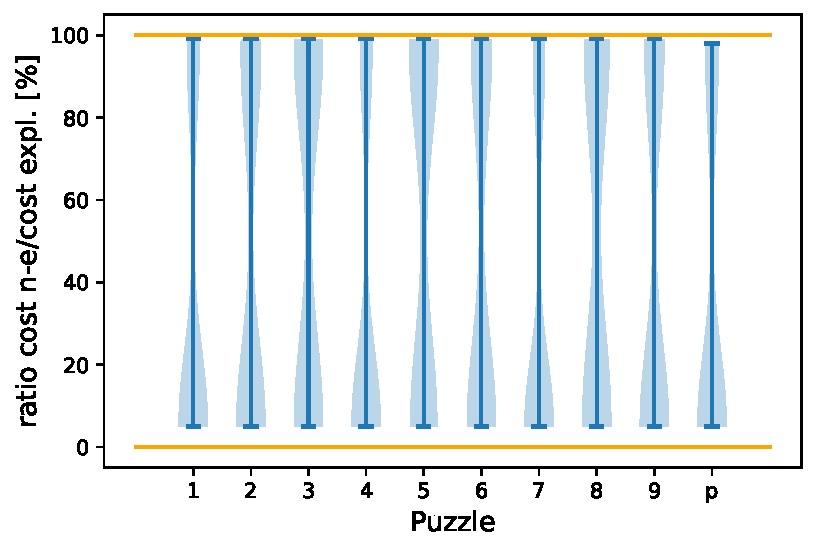
\includegraphics[width=.7\textwidth]{figures/violin_plot.pdf}
	\caption{Distribution of the ratio of the cost of a nested explanation sequence step and the cost of original explanation step for all puzzles}
	% \todo{Y AXIS VALUES? WHERE IS ONE?}
	% \todo{This figure is suddenly twice in here.}
	\label{fig:experiments:violin}
\end{figure}


\begin{figure}[t!]
	\centering
	\begin{subfigure}{.5\textwidth}
		\centering
		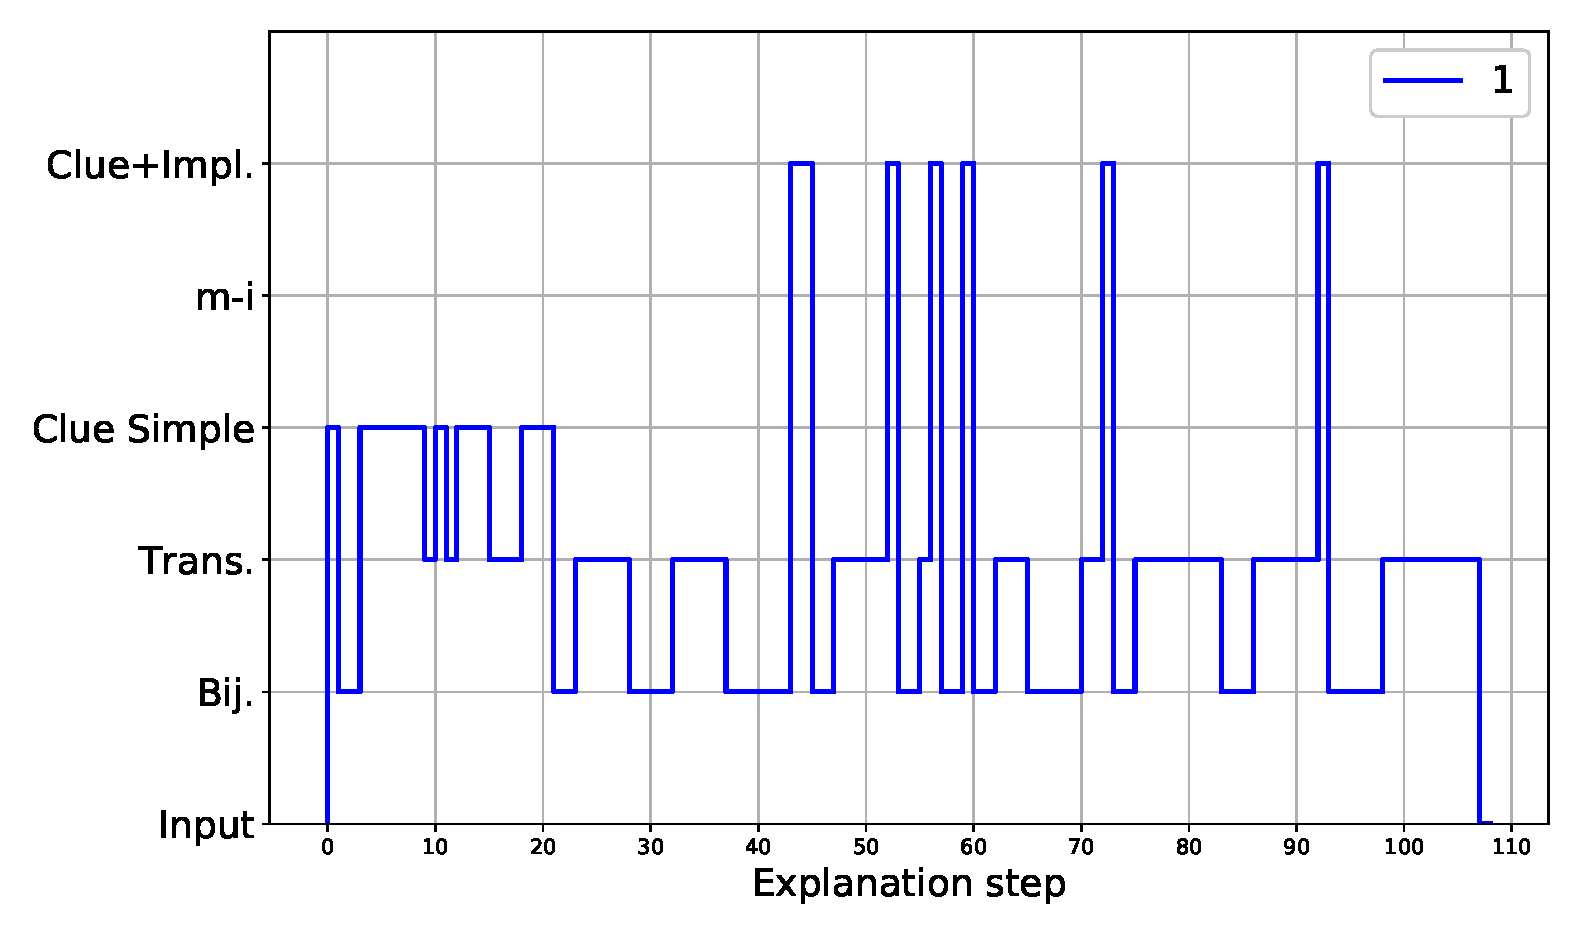
\includegraphics[width=0.9\linewidth]{figures/plot_cost_steps_1.eps}
		\caption{Puzzle 1}
		\label{fig:composition_puzzle:p1}
	\end{subfigure}%
	\begin{subfigure}{.5\textwidth}
		\centering
		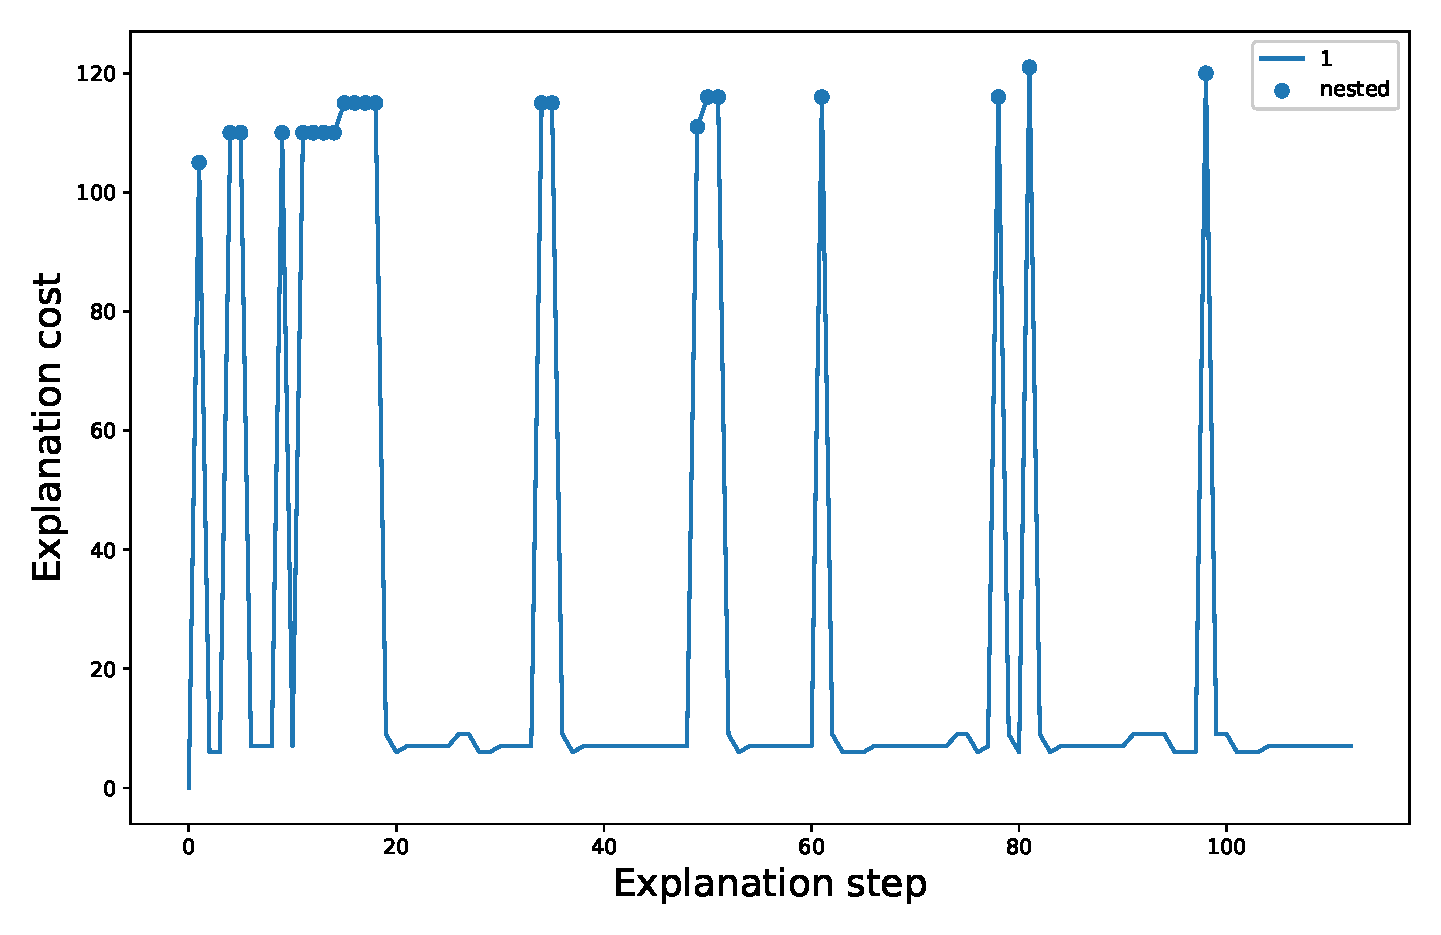
\includegraphics[width=0.84\linewidth]{figures/1.eps}
		\caption{Puzzle 1}
		\label{fig:cost_puzzle:p1}
	\end{subfigure}
	\begin{subfigure}{.5\textwidth}
		\centering
		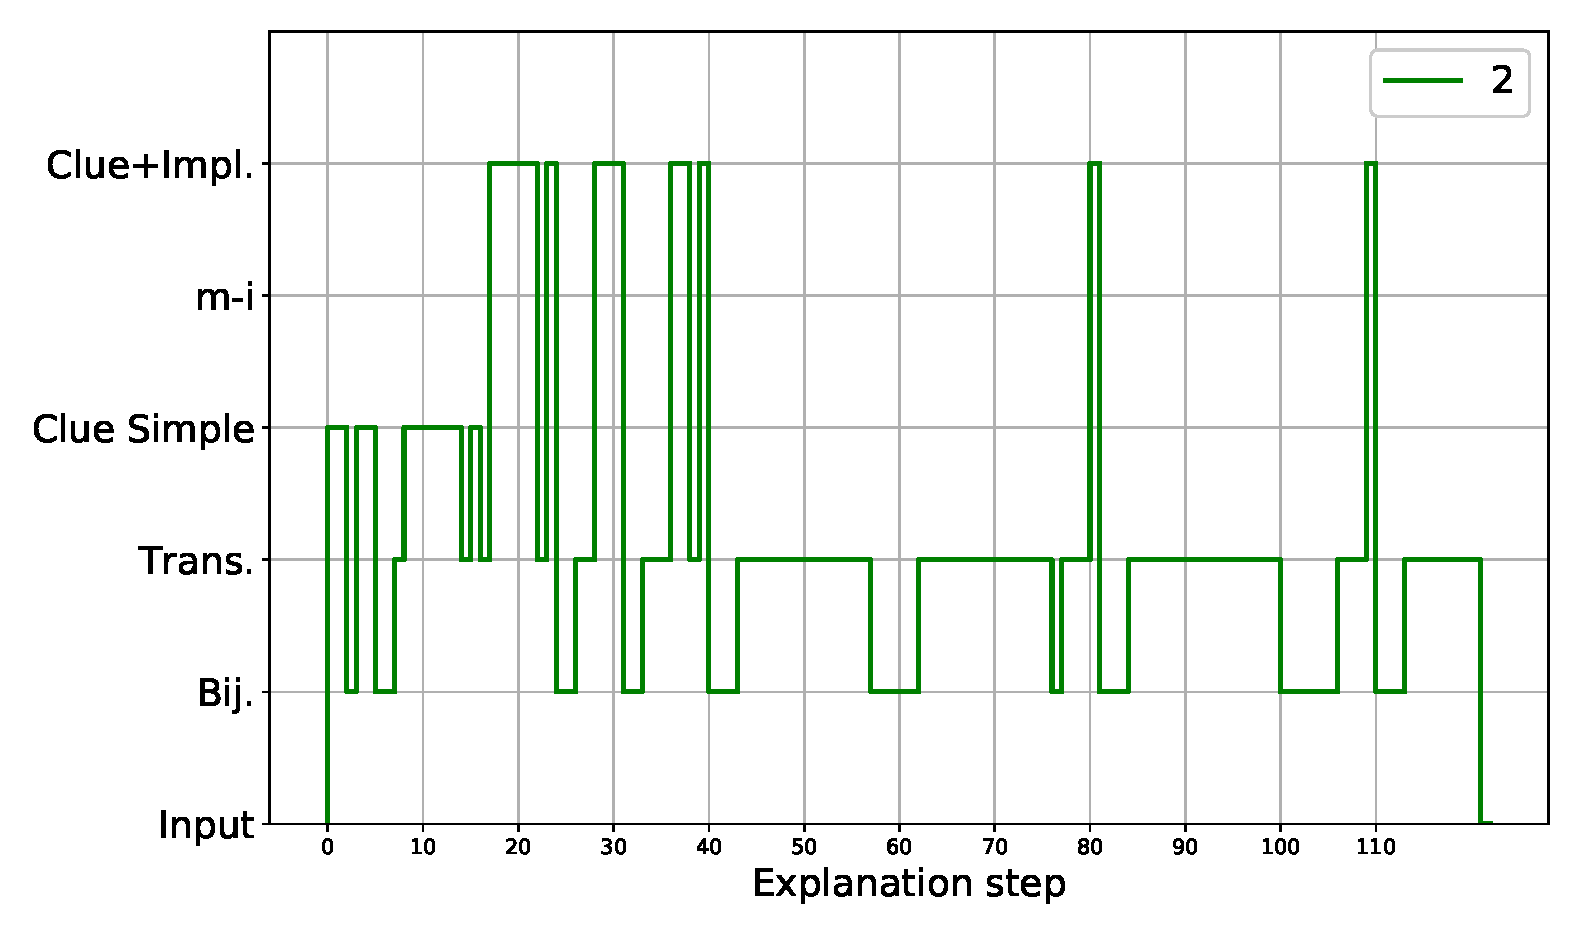
\includegraphics[width=0.9\linewidth]{figures/plot_cost_steps_2.eps}
		\caption{Puzzle 2}
		\label{fig:composition_puzzle:p2}
	\end{subfigure}%
	\begin{subfigure}{.5\textwidth}
		\centering
		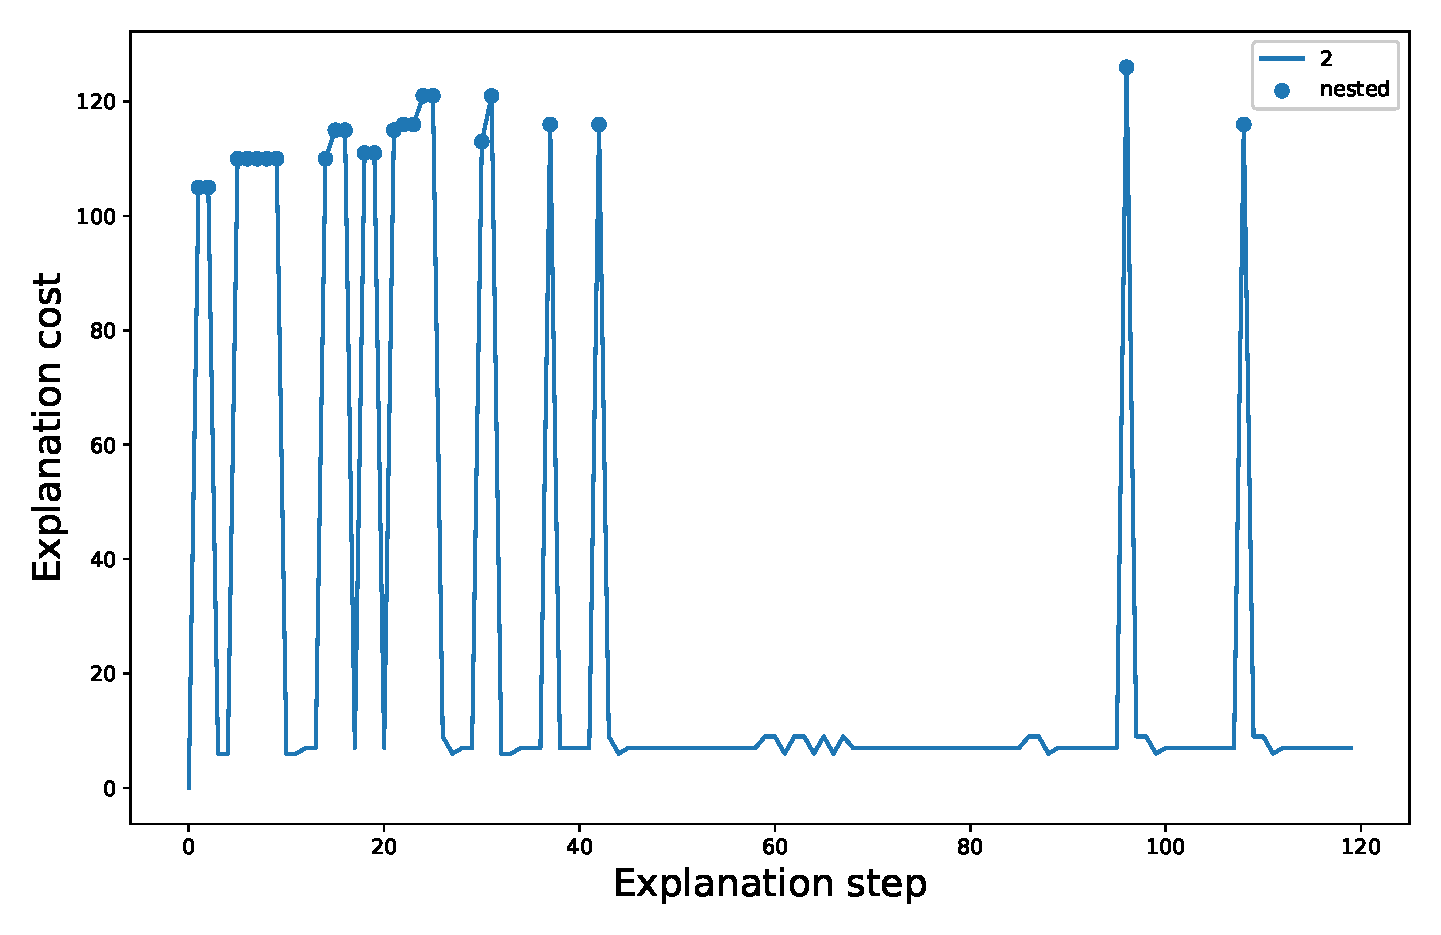
\includegraphics[width=0.84\linewidth]{figures/2.eps}
		\caption{Puzzle 2}
		\label{fig:cost_puzzle:p2}
	\end{subfigure}
	\begin{subfigure}{.5\textwidth}
		\centering
		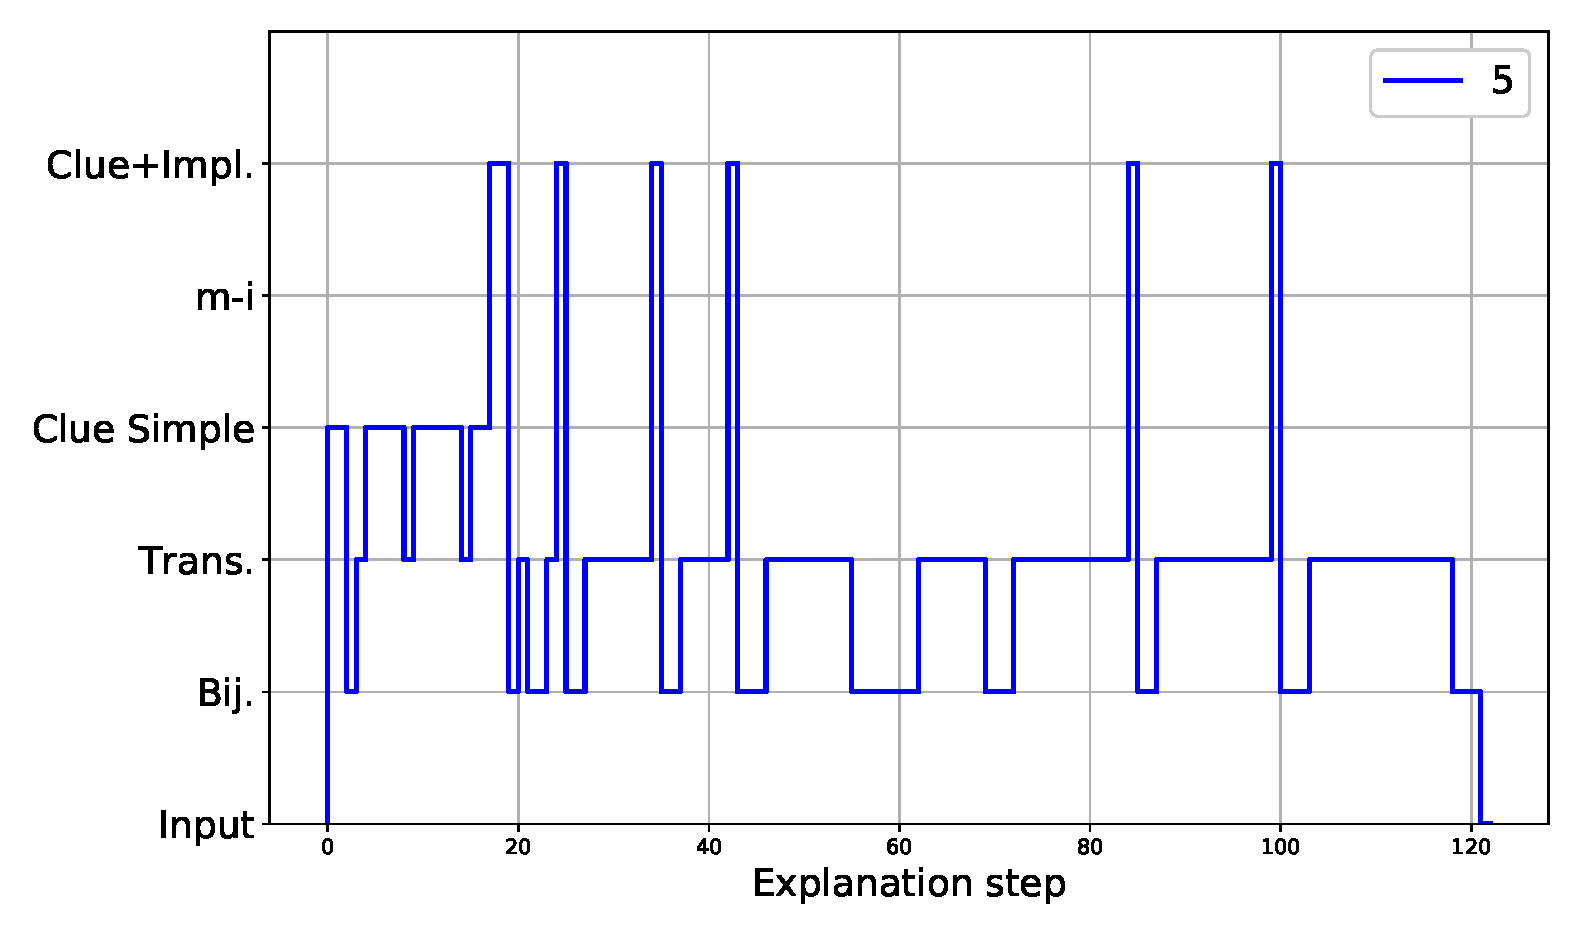
\includegraphics[width=0.9\linewidth]{figures/plot_cost_steps_5.eps}
		\caption{Puzzle 5}
		\label{fig:composition_puzzle:p5}
	\end{subfigure}%
	\begin{subfigure}{.5\textwidth}
		\centering
		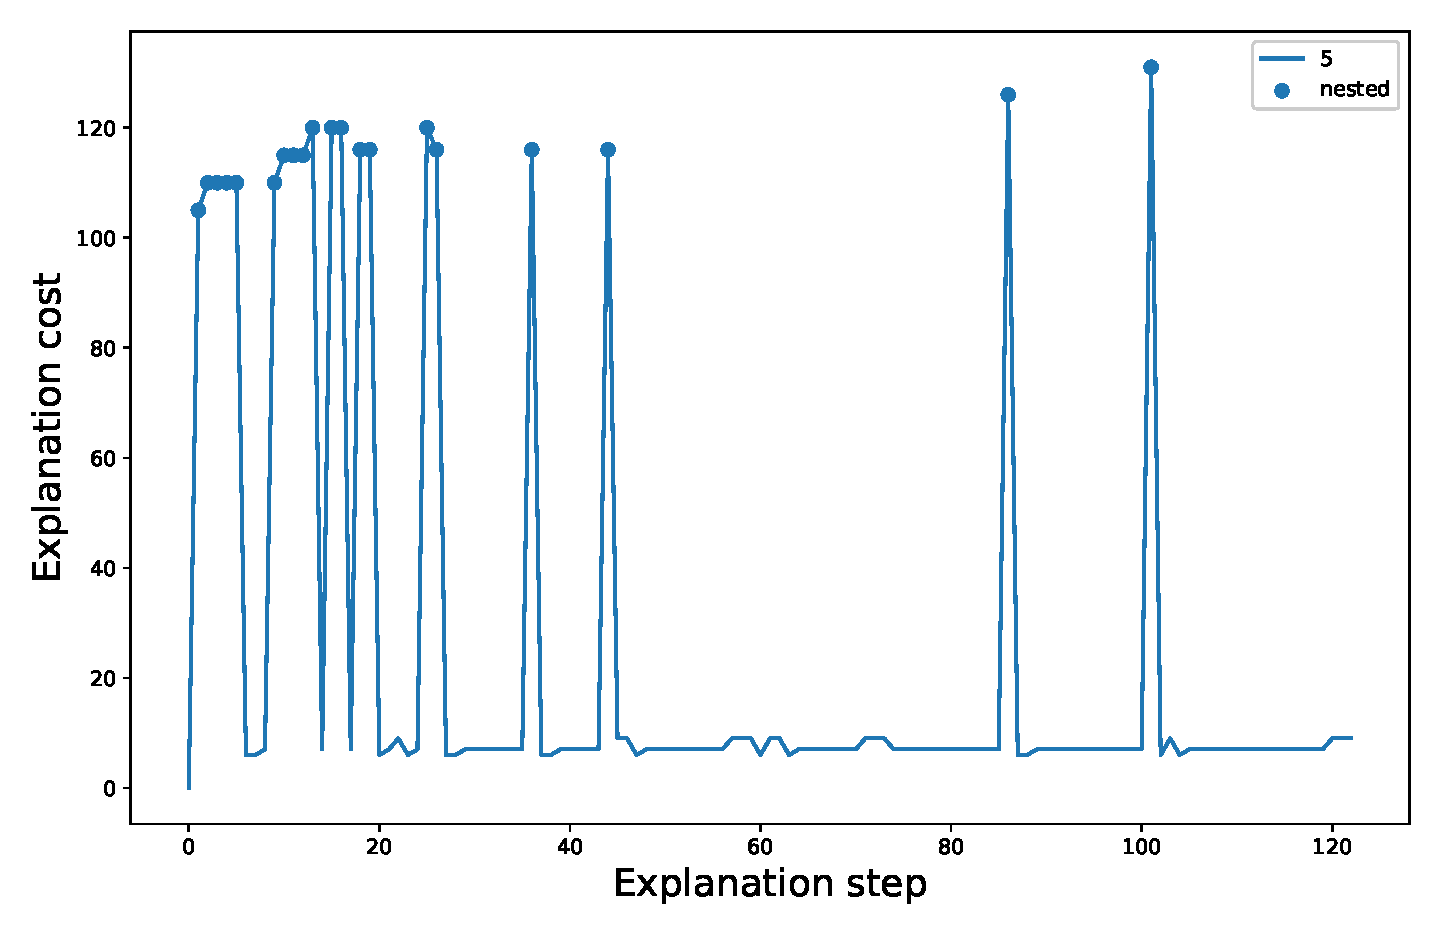
\includegraphics[width=0.84\linewidth]{figures/5.eps}
		\caption{Puzzle 5 }
		\label{fig:cost_puzzle:p5}
	\end{subfigure}
	\begin{subfigure}{.5\textwidth}
		\centering
		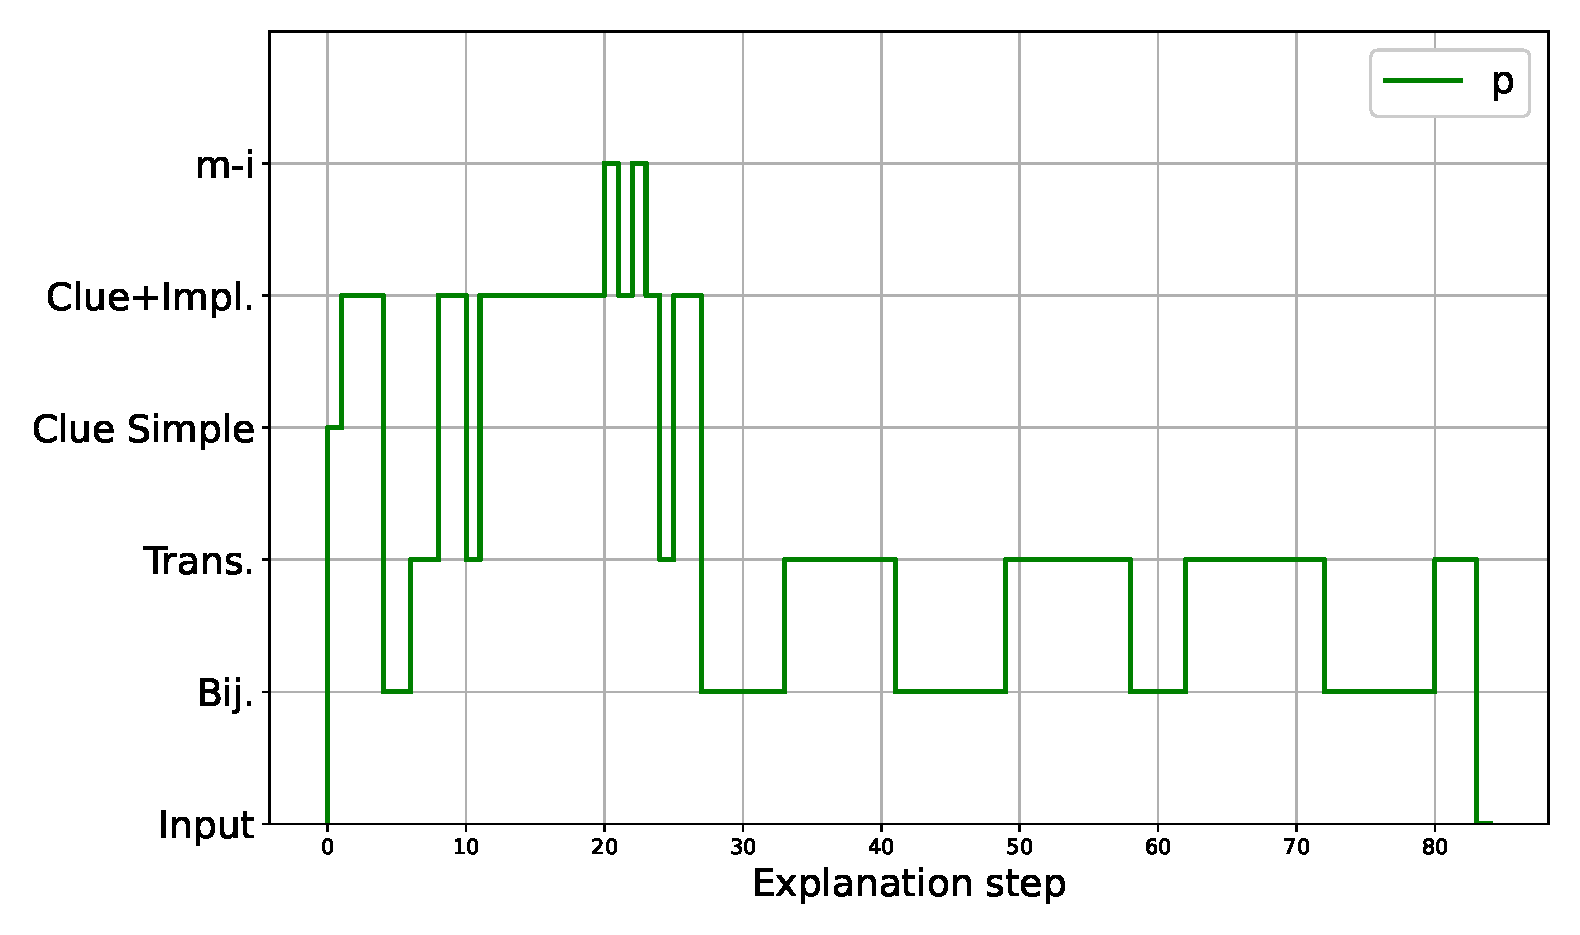
\includegraphics[width=0.9\linewidth]{figures/plot_cost_steps_p.eps}
		\caption{Pasta puzzle}
		\label{fig:composition_puzzle:pasta}
	\end{subfigure}%
	\begin{subfigure}{.5\textwidth}
		\centering
		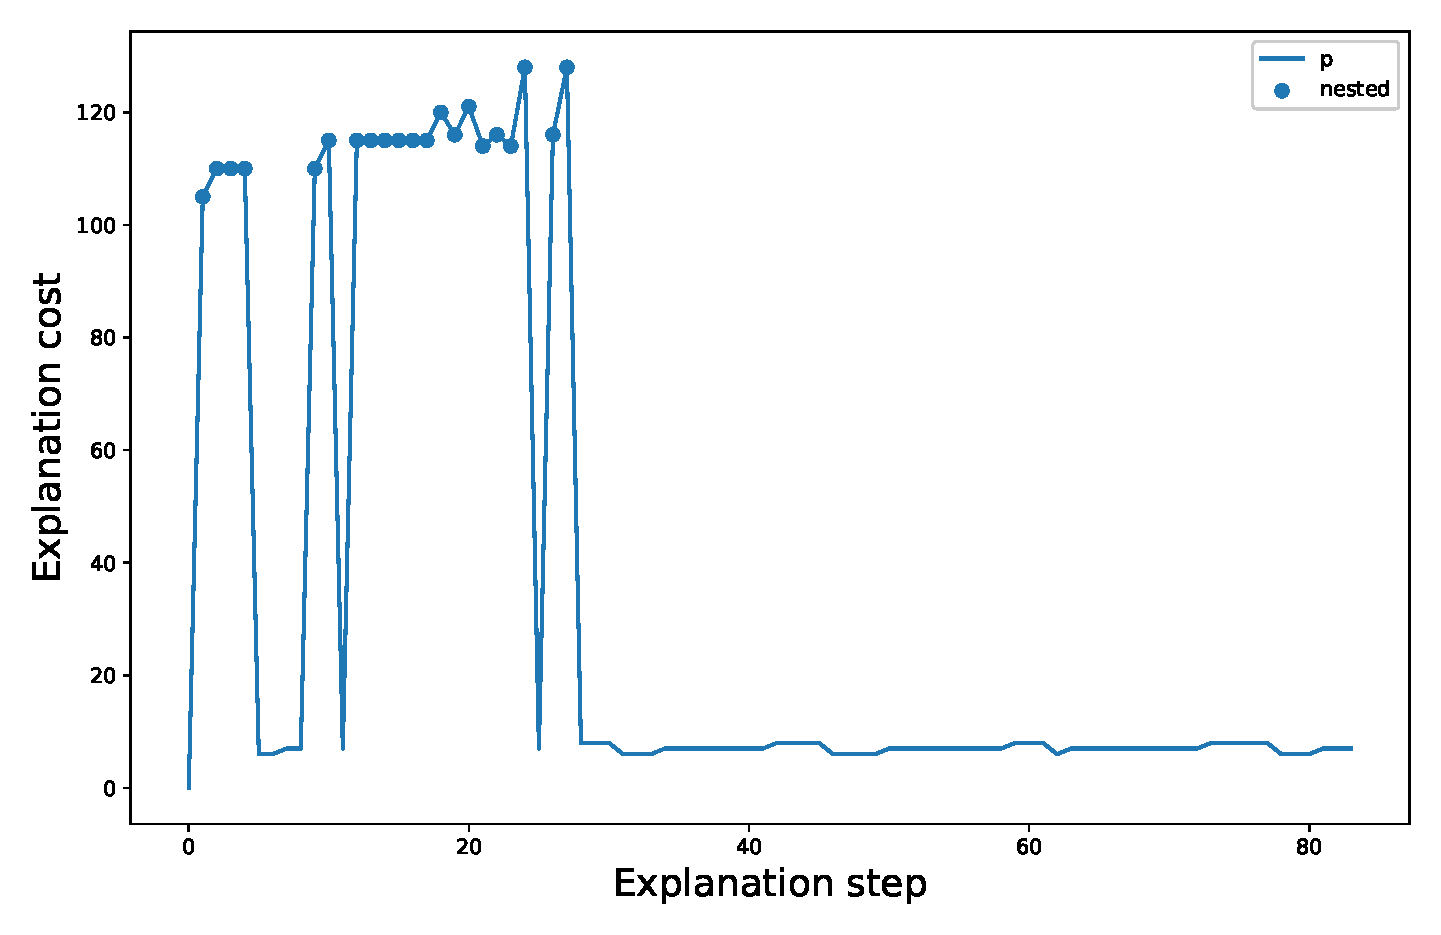
\includegraphics[width=0.84\linewidth]{figures/p.eps}
		\caption{Pasta puzzle}
		\label{fig:cost_puzzle:pasta}
	\end{subfigure}
	\caption{Side-by-side comparison of puzzle composition (left) and puzzle complexity with nested explanation steps highlighted (right)}
	\label{fig:steps}
\end{figure}
% \begin{landscape}
% \begin{table}[t]
% 	\centering
% 	\begin{tabular}{c|cc|cc|c|ccccc}
% 		           &                    & \textbf{\% nested} & \multicolumn{2}{c|}{\textbf{\% non-trivial steps}} & \multicolumn{1}{c|}{\textbf{avg n.-e.}} & \multicolumn{5}{c}{\textbf{Composition of nested explanation (n.-e.)}}                                                                                       \\
% 		\textbf{p} & \textbf{\# steps } & \textbf{steps}     & \textbf{clues+i-c.}                                & \textbf{m-i}          & \textbf{\#steps}                  & \textbf{Bij.} & \textbf{Trans.} & \textbf{Clue} & \textbf{Clue+i-c.} & \textbf{m-i} \\\hline
% 		1 &      112 &  14.29\% &  100.00\% &  0.00\% &         3.00 &  36.99\% &   32.88\% &  12.33\% &    17.81\% &    0.00\% \\
% 		2 &      119 &  14.29\% &  100.00\% &  0.00\% &         3.00 &  48.28\% &   10.34\% &  20.69\% &    20.69\% &    0.00\% \\
% 		3 &      110 &   7.27\% &  100.00\% &  0.00\% &         2.00 &  50.00\% &    0.00\% &   0.00\% &    50.00\% &    0.00\% \\
% 		4 &      115 &  13.04\% &  100.00\% &  0.00\% &         4.00 &  40.26\% &   29.87\% &  20.78\% &     9.09\% &    0.00\% \\
% 		5 &      122 &  13.11\% &  100.00\% &  0.00\% &         2.00 &  47.83\% &    0.00\% &   8.70\% &    43.48\% &    0.00\% \\
% 		6 &      115 &  10.43\% &  100.00\% &  0.00\% &         3.00 &  50.00\% &    8.00\% &  20.00\% &    22.00\% &    0.00\% \\
% 		7 &      110 &  15.45\% &  100.00\% &  0.00\% &         3.00 &  37.50\% &   32.69\% &  18.27\% &    11.54\% &    0.00\% \\
% 		8 &      118 &   9.32\% &  100.00\% &  0.00\% &         2.00 &  43.75\% &    9.38\% &  25.00\% &    21.88\% &    0.00\% \\
% 		9 &      114 &  10.53\% &  100.00\% &  0.00\% &         4.00 &  31.25\% &   28.12\% &  20.31\% &    20.31\% &    0.00\% \\
% 		p &       83 &  16.87\% &   90.48\% &  9.52\% &         3.00 &  48.44\% &   20.31\% &   7.81\% &    17.19\% &    6.25\% \\
% 	\end{tabular}
% 	\caption{Puzzle explanation cost based on the cost function $f(I, C)$ and statistics on puzzle constraints}

% 	\label{table:nested_explanation}

% \end{table}
% \end{landscape}


%THIS SERVES TO PUT EVERYTHING IN THE RIGHT ORDER AS IT IS MENTIONED: FIRST THE TABLE.}
% old?
%\newcommand\ourfigure{
%\begin{figure}[t!]
%	\centering
%	\begin{subfigure}{.5\textwidth}
%		\centering
%		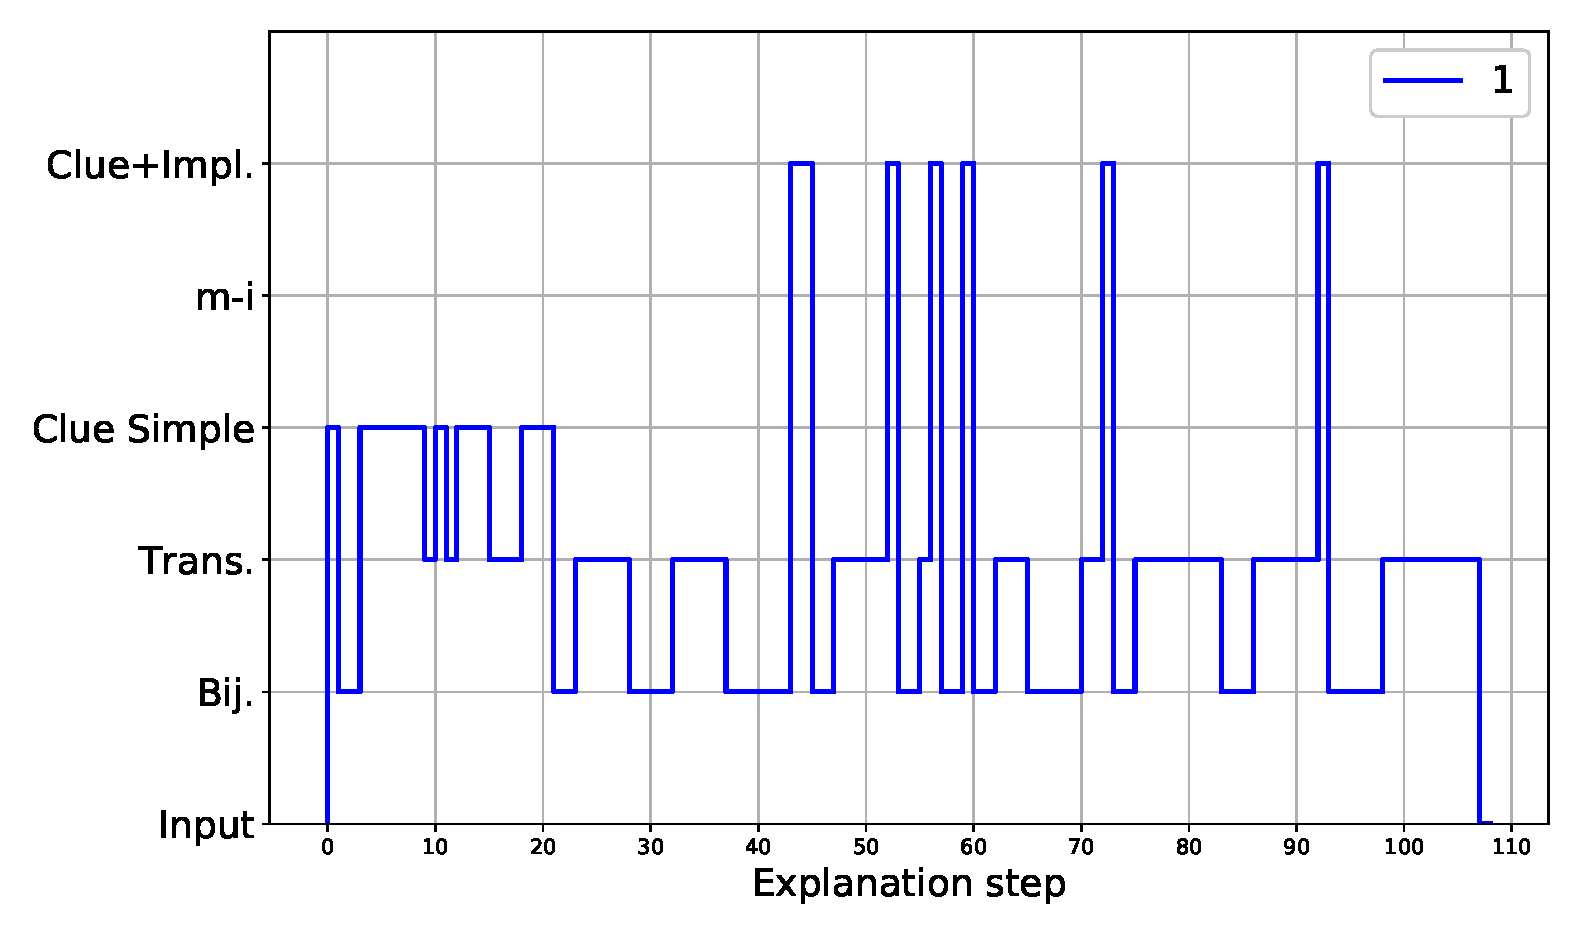
\includegraphics[width=0.98\linewidth]{figures/plot_cost_steps_1.eps}
%		\caption{A subfigure}
%% 		\label{fig:sub1} %I REMOVED THESE SINCE THEY WERE DOUBLE. SHOULD NOT BE REFERRED TO... 
%	\end{subfigure}%
%	\begin{subfigure}{.5\textwidth}
%		\centering
%		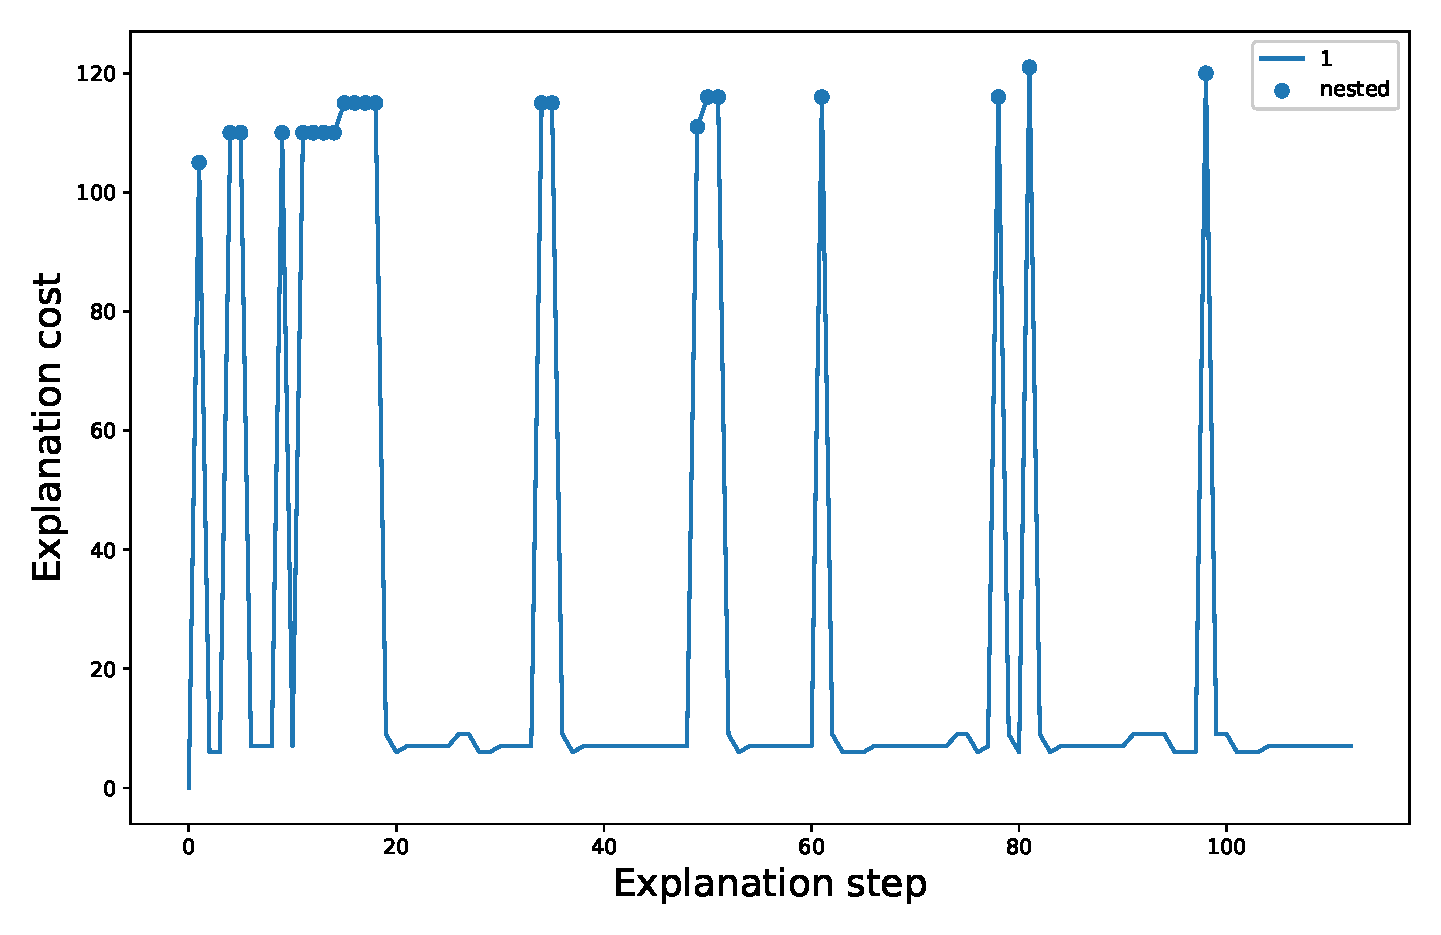
\includegraphics[width=0.9\linewidth]{figures/1.eps}
%		\caption{A subfigure}
%% 		\label{fig:sub2}
%	\end{subfigure}
%	\begin{subfigure}{.5\textwidth}
%		\centering
%		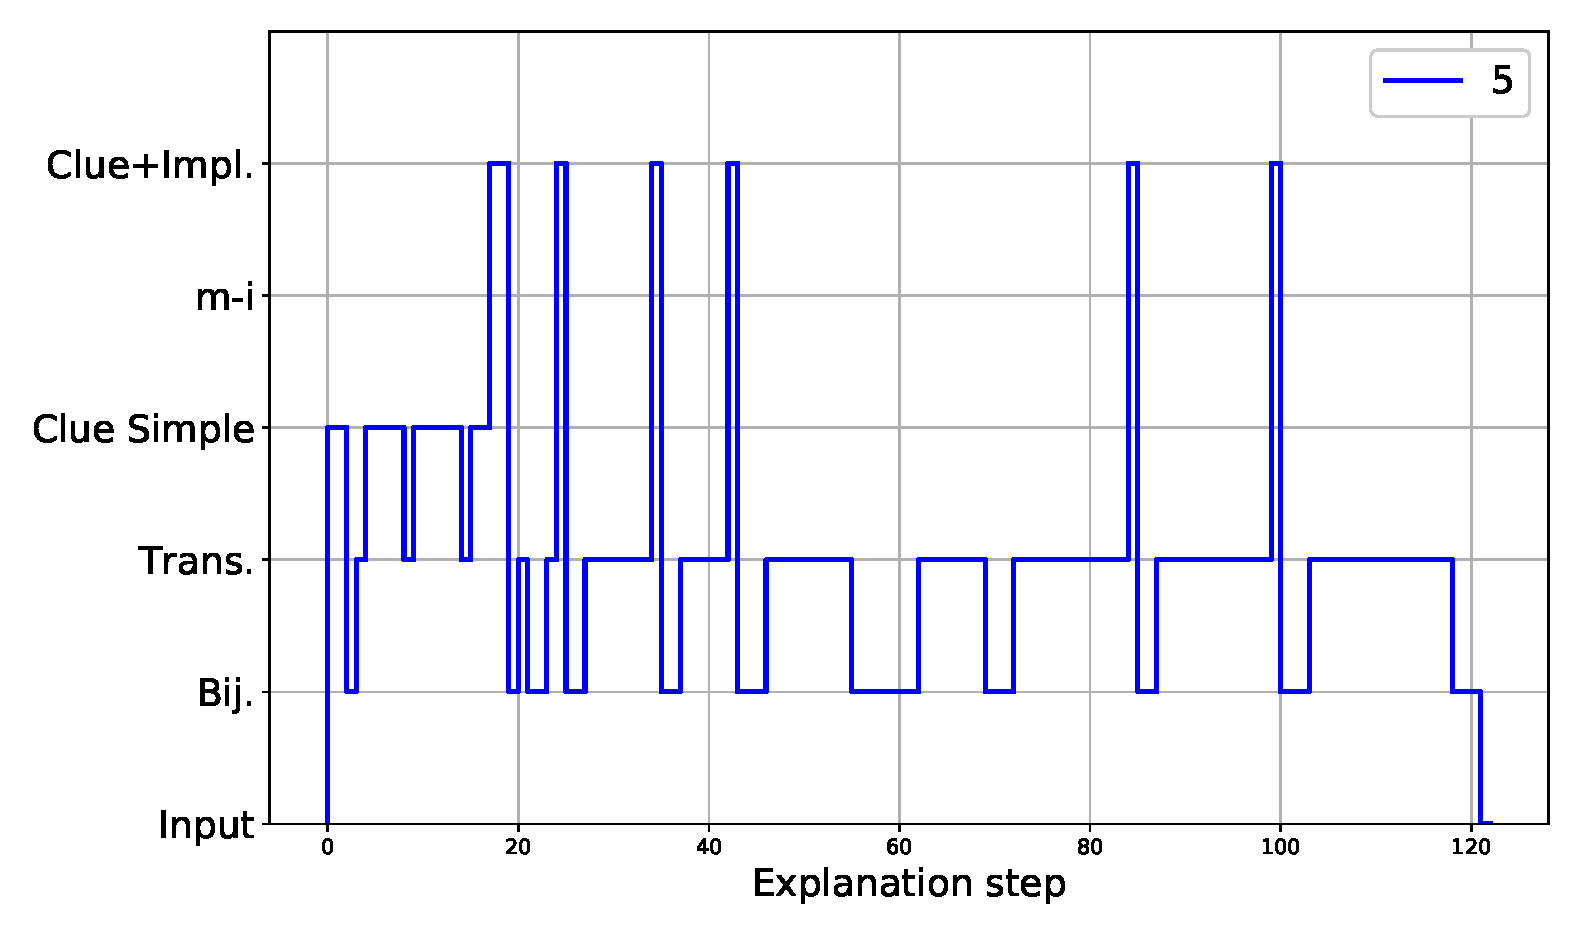
\includegraphics[width=0.98\linewidth]{figures/plot_cost_steps_5.eps}
%		\caption{A subfigure}
%% 		\label{fig:sub1}
%	\end{subfigure}%
%	\begin{subfigure}{.5\textwidth}
%		\centering
%		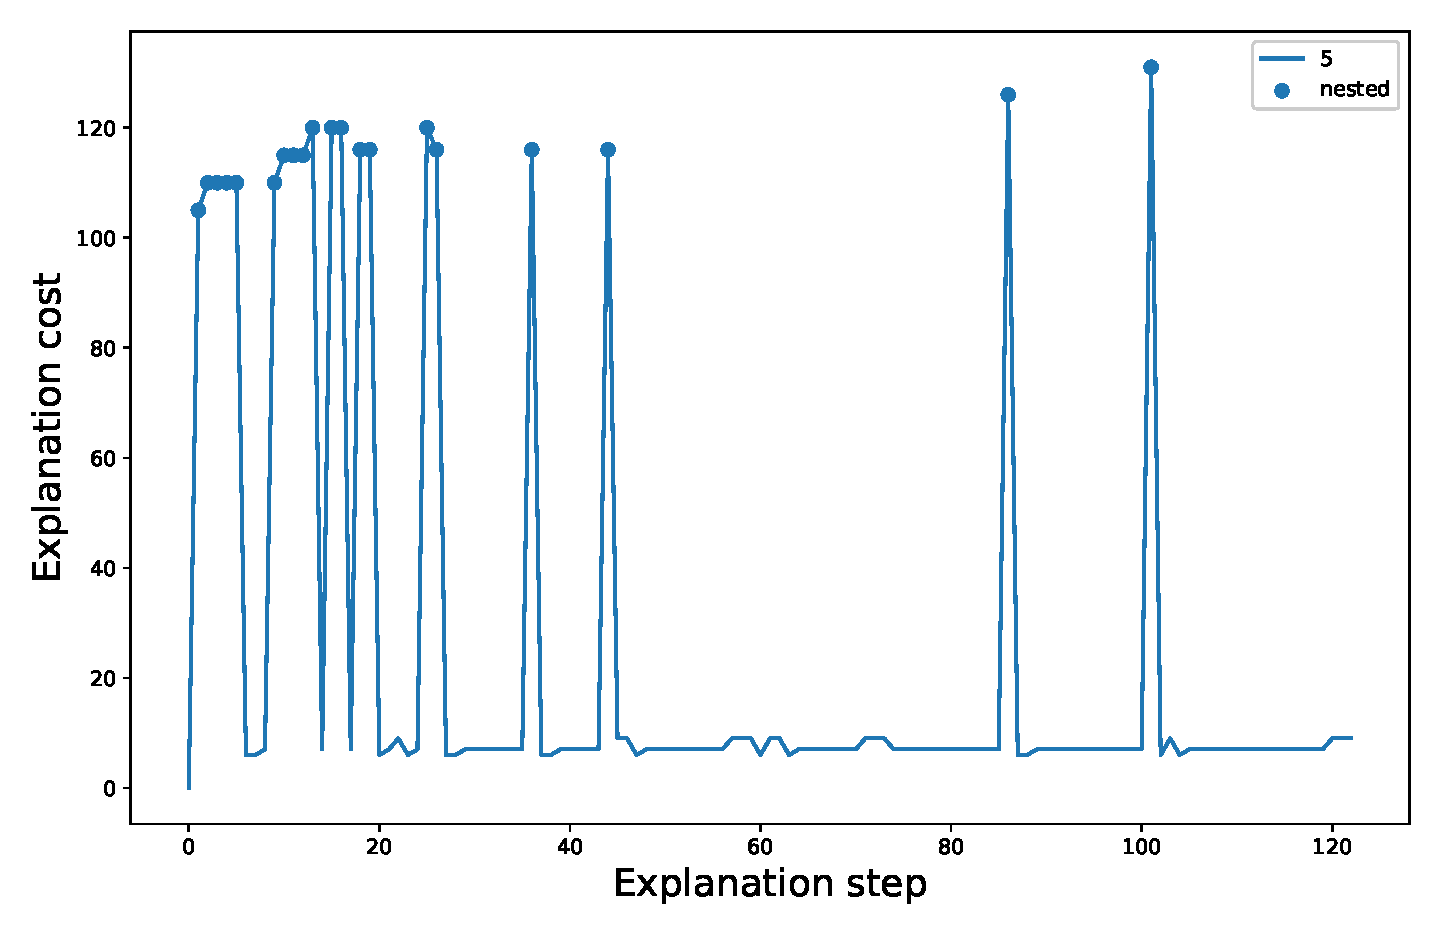
\includegraphics[width=0.9\linewidth]{figures/5.eps}
%		\caption{A subfigure}
%% 		\label{fig:sub2}
%	\end{subfigure}
%	\begin{subfigure}{.5\textwidth}
%		\centering
%		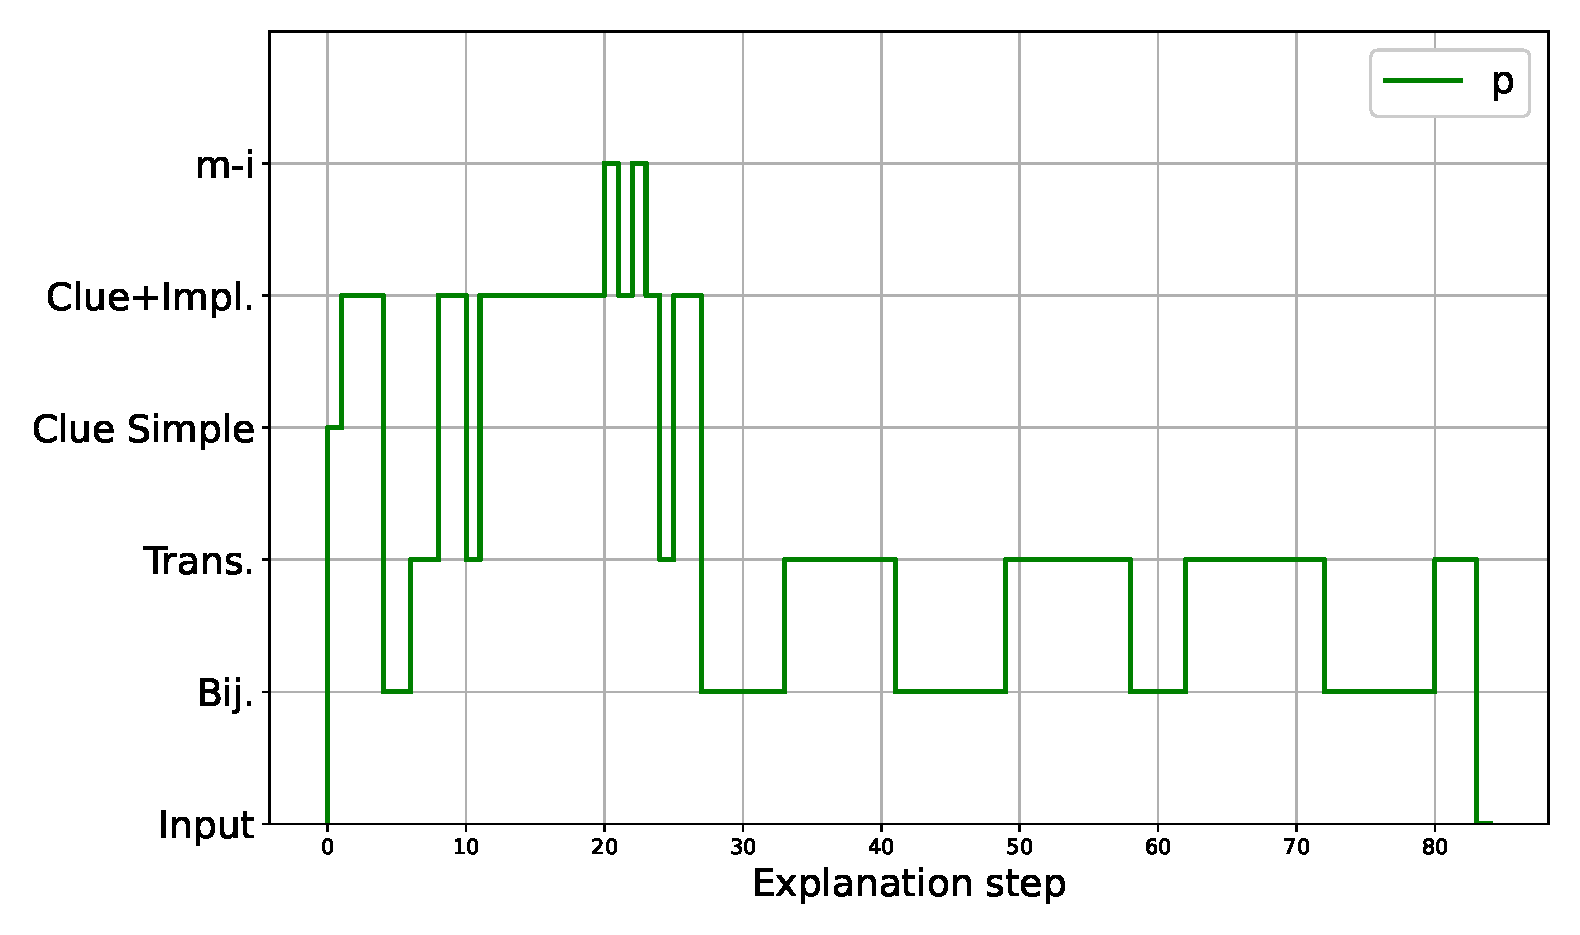
\includegraphics[width=0.98\linewidth]{figures/plot_cost_steps_p.eps}
%		\caption{A subfigure}
%% 		\label{fig:sub1}
%	\end{subfigure}%
%	\begin{subfigure}{.5\textwidth}
%		\centering
%		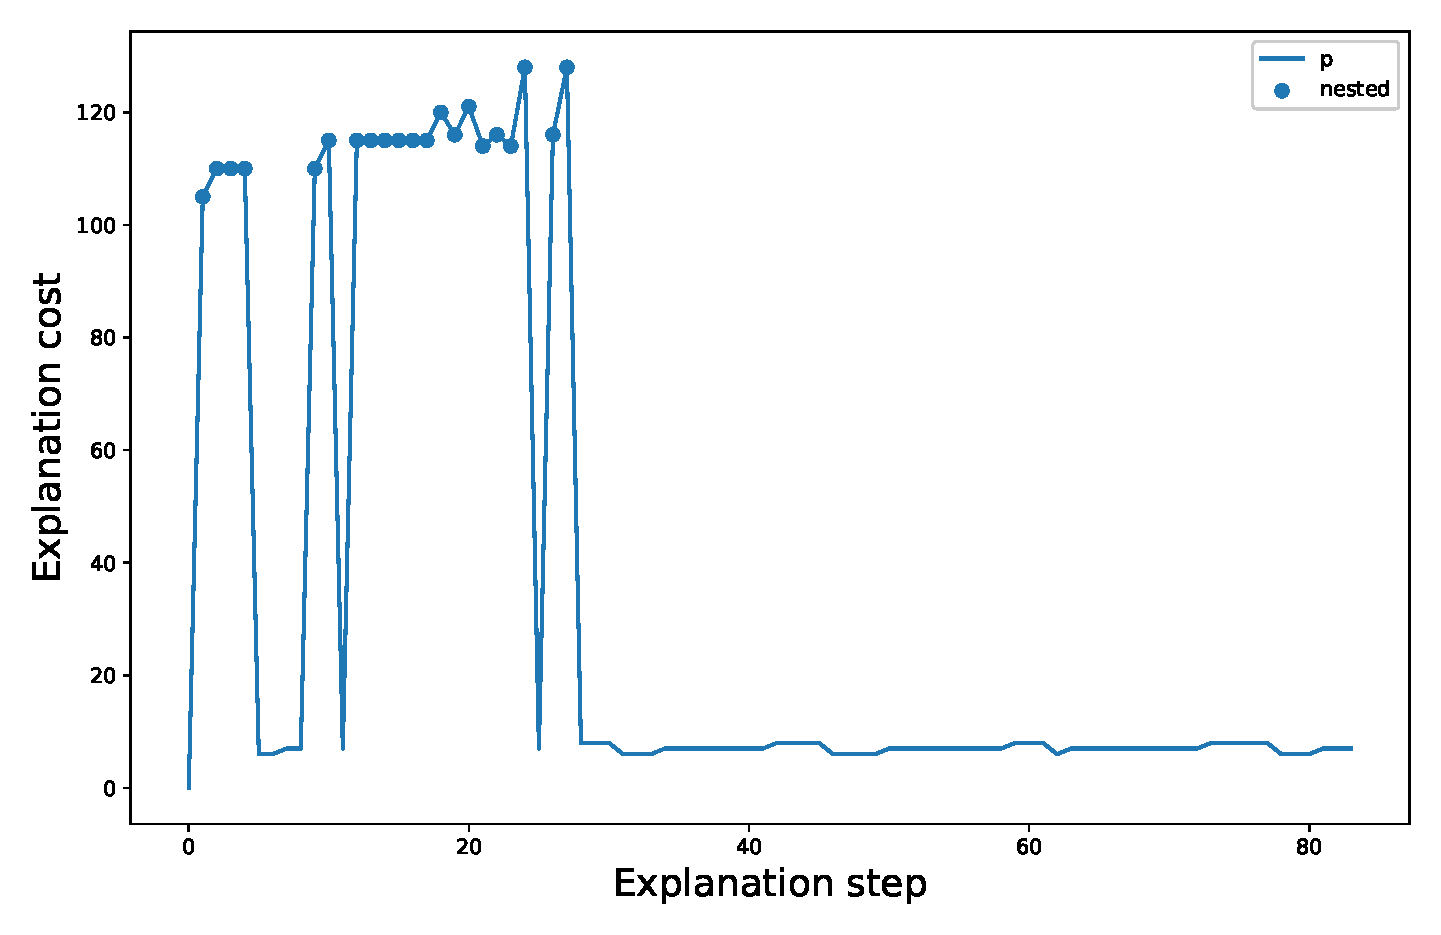
\includegraphics[width=0.9\linewidth]{figures/p.eps}
%		\caption{A subfigure}
%% 		\label{fig:sub2}
%	\end{subfigure}
%	\caption{A figure with two subfigures}
%	%\label{fig:steps}
%\end{figure}
%}

% \begin{table}[b]
% 	\centering
% 	% 	\resizebox{\textwidth}{!}{%
% 	\begin{tabular}{c|c|cc|cccccc}
% 		\textbf{p} & \textbf{($|$types$|$, $|$dom$|$, $|$grid$|$)} & \textbf{\# steps} & $\overline{\text{\textbf{cost}}}$ & \textbf{1 bij.} & \textbf{1 trans.} & \textbf{1 clue} & \textbf{1 clue+1i. (+$>$1i.)} & \textbf{mult i.} & \textbf{mult c.} \\\hline
% 		% \textbf{p} & \textbf{$|$types$|$, $|$dom$|$, $|$grid$|$} & \textbf{\# steps} & $\overline{\text{\textbf{cost}}}$ & \textbf{1 bij.} & \textbf{1 trans.} & \textbf{1 clue} & \textbf{1 clue+1i.} & \textbf{1 clue+ $>$1i.} & \textbf{mult i.} & \textbf{mult c.} \\\hline
% 		1 &       (4, 5, 150) &    112 &      27.06 &  31.25\% &  50.00\% &         0.89\% &      7.14\%  (+10.71\% ) &  0.00\%  &  0.00\%  \\
% 		2 &       (4, 5, 150) &    119 &      27.77 &  23.53\% &  57.14\% &         1.68\% &      7.56\%  (+10.08\% ) &  0.00\%  &  0.00\%  \\
% 		3 &       (4, 5, 150) &    110 &      23.93 &  32.73\% &  51.82\% &         0.00\% &      2.73\%  (+12.73\% ) &  0.00\%  &  0.00\%  \\
% 		4 &       (4, 5, 150) &    115 &      24.54 &  27.83\% &  55.65\% &         2.61\% &      7.83\%  (+ 6.09\% ) &  0.00\%  &  0.00\%  \\
% 		5 &       (4, 5, 150) &    122 &      24.97 &  24.59\% &  59.02\% &         0.82\% &      4.10\%  (+11.48\% ) &  0.00\%  &  0.00\%  \\
% 		6 &       (4, 5, 150) &    115 &      22.58 &  26.96\% &  58.26\% &         2.61\% &      6.09\%  (+ 6.09\% ) &  0.00\%  &  0.00\%  \\
% 		7 &       (4, 5, 150) &    110 &      26.79 &  35.45\% &  46.36\% &         0.91\% &      8.18\%  (+ 9.09\% ) &  0.00\%  &  0.00\%  \\
% 		8 &       (4, 5, 150) &    118 &      26.81 &  33.90\% &  47.46\% &         3.39\% &      5.08\%  (+10.17\% ) &  0.00\%  &  0.00\%  \\
% 		9 &       (4, 5, 150) &    114 &      24.75 &  28.95\% &  54.39\% &         3.51\% &      3.51\%  (+ 9.65\% ) &  0.00\%  &  0.00\%  \\
% 		p &       (4, 4, 96\ ) &     83 &      34.45 &  33.73\% &  40.96\% &         1.20\% &      4.82\% (+ 16.87\%)  &  2.41\%  &  0.00\%
% 	\end{tabular}
% 	% 	}
% 	\caption{Properties of the puzzles, explanation sequences and constraints used in the explanations.}
% 	\label{table:composition}
% \end{table}

% \begin{table}[b]
% 	\centering
% 	% 	\resizebox{\textwidth}{!}{%
% 	\begin{tabular}{c|c|cc|ccccccc}
% 		\textbf{p} & \textbf{($|$types$|$, $|$dom$|$, $|$grid$|$)} & \textbf{\# steps} & $\overline{\text{\textbf{cost}}}$ & \textbf{1 bij.} & \textbf{1 trans.} & \textbf{1 clue} & \textbf{1 clue+1i.} & \textbf{1 clue+ $>$1i.} & \textbf{mult i.} & \textbf{mult c.} \\\hline
% 		% \textbf{p} & \textbf{$|$types$|$, $|$dom$|$, $|$grid$|$} & \textbf{\# steps} & $\overline{\text{\textbf{cost}}}$ & \textbf{1 bij.} & \textbf{1 trans.} & \textbf{1 clue} & \textbf{1 clue+1i.} & \textbf{1 clue+ $>$1i.} & \textbf{mult i.} & \textbf{mult c.} \\\hline
% 		1 &       (4, 5, 150) &    112 &      27.06 &  31.25\% &  50.00\% &         0.89\% &      7.14\% &  10.71\%  &  0.00\%  &  0.00\%  \\
% 		2 &       (4, 5, 150) &    119 &      27.77 &  23.53\% &  57.14\% &         1.68\% &      7.56\% &  10.08\%  &  0.00\%  &  0.00\%  \\
% 		3 &       (4, 5, 150) &    110 &      23.93 &  32.73\% &  51.82\% &         0.00\% &      2.73\% &  12.73\%  &  0.00\%  &  0.00\%  \\
% 		4 &       (4, 5, 150) &    115 &      24.54 &  27.83\% &  55.65\% &         2.61\% &      7.83\% &   6.09\%  &  0.00\%  &  0.00\%  \\
% 		5 &       (4, 5, 150) &    122 &      24.97 &  24.59\% &  59.02\% &         0.82\% &      4.10\% &  11.48\%  &  0.00\%  &  0.00\%  \\
% 		6 &       (4, 5, 150) &    115 &      22.58 &  26.96\% &  58.26\% &         2.61\% &      6.09\% &   6.09\%  &  0.00\%  &  0.00\%  \\
% 		7 &       (4, 5, 150) &    110 &      26.79 &  35.45\% &  46.36\% &         0.91\% &      8.18\% &   9.09\%  &  0.00\%  &  0.00\%  \\
% 		8 &       (4, 5, 150) &    118 &      26.81 &  33.90\% &  47.46\% &         3.39\% &      5.08\% &  10.17\%  &  0.00\%  &  0.00\%  \\
% 		9 &       (4, 5, 150) &    114 &      24.75 &  28.95\% &  54.39\% &         3.51\% &      3.51\% &   9.65\%  &  0.00\%  &  0.00\%  \\
% 		p &       (4, 4, 96\ ) &     83 &      34.45 &  33.73\% &  40.96\% &         1.20\% &      4.82\% &  16.87\%  &  2.41\%  &  0.00\%
% 	\end{tabular}
% 	% 	}
% 	\caption{Properties of the puzzles, explanation sequences and constraints used in the explanations.}
% 	\label{table:composition}
% \end{table}